We demonstrate the network guided estimator and examine its small-sample performance using the following simple simulations. First, we consider the case where the true covariance \(\Sigma\) comes from an AR(1) model. So for \(\Bqty{(i,j): i =1 ,\dots, N, j = 1,\dots,N} \), \(\sigma_{ij}^{2} = \sigma_{i}\sigma_{j} \rho_{ij}\) and \(\rho_{ij} = \rho^{\abs{i - j}}\). We take \(N = 400\). 
\begin{equation*}
     S_{ij} = 3 * \rho^{\abs{i - j}}
\end{equation*}
and assume we observe a matrix \(G(l)\) indicating the location of highly correlated pairs \(L_{ij}(l) = \mathbf{1}\Bqty{\rho_{ij} \geq l}\). Conditional on \(L_{ij} = 1\), we observe \(G_{ij}= 1\) with probability \(p\) and conditional on \(L_{ij}  =0\) , \(G_{ij}  =1\) with probability \(q\). Hence \(p,q\) reflect the probability of missing important locations and including false important locations respectively. 

We then generate \(T = 100\) independent drws of observations \(X \sim N(0, \Sigma)\) and estimate \(\Sigma\) using 
\begin{enumerate*}
     \item Sample covariance ;
     \item Linear Shrinkage estimator;
     \item Nonlinear Shrinkage estimator;
     \item Universal thresholding on the correlation;
     \item and Network Guided thresholding estimator. 
\end{enumerate*}
We now compare their performance. It's worth collecting here the parameters that we will adjust in the experiments:
\begin{table}[htbp]
     \centering\begin{tabularx}{\textwidth}{c|X}
          \toprule
          Parameter & Description \\ 
          \midrule
          \(\rho\) & Determines how strong the correlation is and the sparsity of the covariance matrix \(\Sigma\) \\
          \(l\) & Observation level, determines how we classify a pair \((i,j)\) as important, i.e., \(L_{ij} =1\). \\
          \(p\) & Conditional on \(L_{ij} =1\), the probability of actually observing \(G_{ij} =1\). \\
          \(q\) & Conditional on \(L_{ij} = 0\), the probability of  observing \(G_{ij} =1\)\\
          \(\tau\)& The Threshold level when we apply generalized thresholding operator on \(\sigma_{ij}\) where \(G_{ij} = 0\). \\
          \bottomrule
     \end{tabularx}
     \caption{Description of varying parameters.}
     \label{t:1}
\end{table}

\begin{longtable}{lp{2cm}|p{2cm}p{2cm}p{2cm}p{2cm}p{2cm}}
\caption{The estimation error of various estimators in terms of the Frobenius Norm}
\label{t:2-fro}\\
\toprule
     &     &  Sample Cov &  Linear Shrinkage &  Nonlinear Shrinkage &  Universal Threshold &  Network Guided \\
\(\rho\) & Threshold Level &             &                   &                      &                      &                 \\
\midrule
\endfirsthead
\caption[]{The estimation error of various estimators in terms of the Frobenius Norm} \\
\toprule
     &     &  Sample Cov &  Linear Shrinkage &  Nonlinear Shrinkage &  Universal Threshold &  Network Guided \\
\(\rho\) & Threshold Level &             &                   &                      &                      &                 \\
\midrule
\endhead
\midrule
\multicolumn{7}{r}{{Continued on next page}} \\
\midrule
\endfoot

\bottomrule
\endlastfoot
0.70 & 0.0 &       59.43 &             42.23 &                41.61 &                59.43 &           59.43 \\
     & 0.1 &       59.43 &             42.23 &                41.61 &                49.91 &           49.85 \\
     & 0.2 &       59.43 &             42.23 &                41.61 &                41.94 &           41.67 \\
     & 0.3 &       59.43 &             42.23 &                41.61 &                35.66 &           34.97 \\
     & 0.4 &       59.43 &             42.23 &                41.61 &                31.20 &           29.81 \\
     & 0.5 &       59.43 &             42.23 &                41.61 &                28.56 &           26.18 \\
     & 0.6 &       59.43 &             42.23 &                41.61 &                27.54 &           23.93 \\
     & 0.7 &       59.43 &             42.23 &                41.61 &                27.78 &           22.81 \\
     & 0.8 &       59.43 &             42.23 &                41.61 &                28.83 &           22.48 \\
     & 0.9 &       59.43 &             42.23 &                41.61 &                30.33 &           22.59 \\
     & 1.0 &       59.43 &             42.23 &                41.61 &                32.08 &           22.98 \\
0.80 & 0.0 &       62.54 &             47.59 &                46.59 &                62.54 &           62.54 \\
     & 0.1 &       62.54 &             47.59 &                46.59 &                52.60 &           52.80 \\
     & 0.2 &       62.54 &             47.59 &                46.59 &                44.30 &           44.52 \\
     & 0.3 &       62.54 &             47.59 &                46.59 &                37.89 &           37.85 \\
     & 0.4 &       62.54 &             47.59 &                46.59 &                33.55 &           32.85 \\
     & 0.5 &       62.54 &             47.59 &                46.59 &                31.32 &           29.48 \\
     & 0.6 &       62.54 &             47.59 &                46.59 &                30.95 &           27.58 \\
     & 0.7 &       62.54 &             47.59 &                46.59 &                31.93 &           26.78 \\
     & 0.8 &       62.54 &             47.59 &                46.59 &                33.75 &           26.71 \\
     & 0.9 &       62.54 &             47.59 &                46.59 &                36.02 &           27.05 \\
     & 1.0 &       62.54 &             47.59 &                46.59 &                38.49 &           27.59 \\
0.90 & 0.0 &       63.06 &             53.18 &                52.83 &                63.06 &           63.06 \\
     & 0.1 &       63.06 &             53.18 &                52.83 &                53.98 &           54.60 \\
     & 0.2 &       63.06 &             53.18 &                52.83 &                46.91 &           47.84 \\
     & 0.3 &       63.06 &             53.18 &                52.83 &                42.16 &           42.89 \\
     & 0.4 &       63.06 &             53.18 &                52.83 &                39.78 &           39.67 \\
     & 0.5 &       63.06 &             53.18 &                52.83 &                39.57 &           37.96 \\
     & 0.6 &       63.06 &             53.18 &                52.83 &                41.08 &           37.43 \\
     & 0.7 &       63.06 &             53.18 &                52.83 &                43.74 &           37.69 \\
     & 0.8 &       63.06 &             53.18 &                52.83 &                47.08 &           38.41 \\
     & 0.9 &       63.06 &             53.18 &                52.83 &                50.74 &           39.33 \\
     & 1.0 &       63.06 &             53.18 &                52.83 &                54.57 &           40.32 \\
0.95 & 0.0 &       57.97 &             52.58 &                51.77 &                57.97 &           57.97 \\
     & 0.1 &       57.97 &             52.58 &                51.77 &                51.42 &           52.21 \\
     & 0.2 &       57.97 &             52.58 &                51.77 &                47.65 &           48.39 \\
     & 0.3 &       57.97 &             52.58 &                51.77 &                46.74 &           46.40 \\
     & 0.4 &       57.97 &             52.58 &                51.77 &                48.35 &           45.96 \\
     & 0.5 &       57.97 &             52.58 &                51.77 &                51.82 &           46.66 \\
     & 0.6 &       57.97 &             52.58 &                51.77 &                56.46 &           48.04 \\
     & 0.7 &       57.97 &             52.58 &                51.77 &                61.73 &           49.73 \\
     & 0.8 &       57.97 &             52.58 &                51.77 &                67.33 &           51.51 \\
     & 0.9 &       57.97 &             52.58 &                51.77 &                73.05 &           53.24 \\
     & 1.0 &       57.97 &             52.58 &                51.77 &                78.77 &           54.84 \\
0.99 & 0.0 &      104.67 &            115.10 &               106.32 &               104.67 &          104.67 \\
     & 0.1 &      104.67 &            115.10 &               106.32 &               114.91 &          106.31 \\
     & 0.2 &      104.67 &            115.10 &               106.32 &               125.35 &          108.13 \\
     & 0.3 &      104.67 &            115.10 &               106.32 &               135.88 &          110.08 \\
     & 0.4 &      104.67 &            115.10 &               106.32 &               146.37 &          112.10 \\
     & 0.5 &      104.67 &            115.10 &               106.32 &               156.67 &          114.08 \\
     & 0.6 &      104.67 &            115.10 &               106.32 &               166.73 &          115.97 \\
     & 0.7 &      104.67 &            115.10 &               106.32 &               176.56 &          117.77 \\
     & 0.8 &      104.67 &            115.10 &               106.32 &               186.19 &          119.50 \\
     & 0.9 &      104.67 &            115.10 &               106.32 &               195.60 &          121.16 \\
     & 1.0 &      104.67 &            115.10 &               106.32 &               204.74 &          122.77 \\
\end{longtable}

\begin{longtable}{lp{2cm}|p{2cm}p{2cm}p{2cm}p{2cm}p{2cm}}
\caption{The estimation error of various estimators in terms of the Matrix 1-Norm}
\label{t:2-1}\\
\toprule
     &     &  Sample Cov &  Linear Shrinkage &  Nonlinear Shrinkage &  Universal Threshold &  Network Guided \\
\$rho\$ & Threshold Level &             &                   &                      &                      &                 \\
\midrule
\endfirsthead
\caption[]{The estimation error of various estimators in terms of the Matrix 1-Norm} \\
\toprule
     &     &  Sample Cov &  Linear Shrinkage &  Nonlinear Shrinkage &  Universal Threshold &  Network Guided \\
\$rho\$ & Threshold Level &             &                   &                      &                      &                 \\
\midrule
\endhead
\midrule
\multicolumn{7}{r}{{Continued on next page}} \\
\midrule
\endfoot

\bottomrule
\endlastfoot
0.70 & 0.0 &       70.94 &             36.53 &                36.82 &                70.94 &           70.94 \\
     & 0.1 &       70.94 &             36.53 &                36.82 &                55.93 &           56.28 \\
     & 0.2 &       70.94 &             36.53 &                36.82 &                44.71 &           45.32 \\
     & 0.3 &       70.94 &             36.53 &                36.82 &                34.97 &           35.82 \\
     & 0.4 &       70.94 &             36.53 &                36.82 &                26.96 &           28.05 \\
     & 0.5 &       70.94 &             36.53 &                36.82 &                20.38 &           21.71 \\
     & 0.6 &       70.94 &             36.53 &                36.82 &                16.52 &           17.21 \\
     & 0.7 &       70.94 &             36.53 &                36.82 &                14.44 &           13.75 \\
     & 0.8 &       70.94 &             36.53 &                36.82 &                13.20 &           11.21 \\
     & 0.9 &       70.94 &             36.53 &                36.82 &                12.87 &           10.54 \\
     & 1.0 &       70.94 &             36.53 &                36.82 &                12.67 &           10.18 \\
0.80 & 0.0 &       72.33 &             47.47 &                46.79 &                72.33 &           72.33 \\
     & 0.1 &       72.33 &             47.47 &                46.79 &                59.68 &           60.34 \\
     & 0.2 &       72.33 &             47.47 &                46.79 &                48.53 &           49.80 \\
     & 0.3 &       72.33 &             47.47 &                46.79 &                38.78 &           40.55 \\
     & 0.4 &       72.33 &             47.47 &                46.79 &                30.85 &           32.82 \\
     & 0.5 &       72.33 &             47.47 &                46.79 &                25.75 &           26.66 \\
     & 0.6 &       72.33 &             47.47 &                46.79 &                22.88 &           22.14 \\
     & 0.7 &       72.33 &             47.47 &                46.79 &                21.10 &           18.78 \\
     & 0.8 &       72.33 &             47.47 &                46.79 &                19.92 &           16.11 \\
     & 0.9 &       72.33 &             47.47 &                46.79 &                20.04 &           15.10 \\
     & 1.0 &       72.33 &             47.47 &                46.79 &                20.26 &           14.93 \\
0.90 & 0.0 &       81.75 &             59.18 &                56.66 &                81.75 &           81.75 \\
     & 0.1 &       81.75 &             59.18 &                56.66 &                68.10 &           70.18 \\
     & 0.2 &       81.75 &             59.18 &                56.66 &                57.16 &           61.33 \\
     & 0.3 &       81.75 &             59.18 &                56.66 &                48.38 &           54.47 \\
     & 0.4 &       81.75 &             59.18 &                56.66 &                40.41 &           48.40 \\
     & 0.5 &       81.75 &             59.18 &                56.66 &                33.92 &           43.81 \\
     & 0.6 &       81.75 &             59.18 &                56.66 &                33.02 &           40.06 \\
     & 0.7 &       81.75 &             59.18 &                56.66 &                33.81 &           36.64 \\
     & 0.8 &       81.75 &             59.18 &                56.66 &                35.11 &           33.87 \\
     & 0.9 &       81.75 &             59.18 &                56.66 &                36.60 &           32.95 \\
     & 1.0 &       81.75 &             59.18 &                56.66 &                38.18 &           33.58 \\
0.95 & 0.0 &       80.91 &             79.60 &                77.41 &                80.91 &           80.91 \\
     & 0.1 &       80.91 &             79.60 &                77.41 &                75.95 &           72.89 \\
     & 0.2 &       80.91 &             79.60 &                77.41 &                73.70 &           67.96 \\
     & 0.3 &       80.91 &             79.60 &                77.41 &                73.60 &           64.99 \\
     & 0.4 &       80.91 &             79.60 &                77.41 &                73.83 &           62.35 \\
     & 0.5 &       80.91 &             79.60 &                77.41 &                74.22 &           59.86 \\
     & 0.6 &       80.91 &             79.60 &                77.41 &                74.66 &           57.43 \\
     & 0.7 &       80.91 &             79.60 &                77.41 &                75.15 &           55.09 \\
     & 0.8 &       80.91 &             79.60 &                77.41 &                76.05 &           53.21 \\
     & 0.9 &       80.91 &             79.60 &                77.41 &                77.18 &           52.05 \\
     & 1.0 &       80.91 &             79.60 &                77.41 &                78.95 &           52.05 \\
0.99 & 0.0 &      125.39 &            124.68 &               138.13 &               125.39 &          125.39 \\
     & 0.1 &      125.39 &            124.68 &               138.13 &               124.99 &          122.63 \\
     & 0.2 &      125.39 &            124.68 &               138.13 &               124.99 &          119.93 \\
     & 0.3 &      125.39 &            124.68 &               138.13 &               130.98 &          118.03 \\
     & 0.4 &      125.39 &            124.68 &               138.13 &               142.83 &          116.99 \\
     & 0.5 &      125.39 &            124.68 &               138.13 &               154.67 &          116.69 \\
     & 0.6 &      125.39 &            124.68 &               138.13 &               166.26 &          116.43 \\
     & 0.7 &      125.39 &            124.68 &               138.13 &               177.31 &          117.24 \\
     & 0.8 &      125.39 &            124.68 &               138.13 &               188.01 &          118.44 \\
     & 0.9 &      125.39 &            124.68 &               138.13 &               198.11 &          119.68 \\
     & 1.0 &      125.39 &            124.68 &               138.13 &               207.97 &          120.93 \\
\end{longtable}

In \autoref{t:2-fro}, we show the general performance of these estimators when we simulate using different \(\rho\) and thresholding level \(\tau\). Here we have taken the thresholding operator to be soft thresholding. It can be seen that generally speaking, when the covariance matrix becomes denser, linear, nonlinear shrinakge estimators and the sample covariance estimator become superiro to 

Then we consider simulations with varying observation levels \(l\). In \autoref{fig:1}
\begin{figure}[htbp]
     \centering
     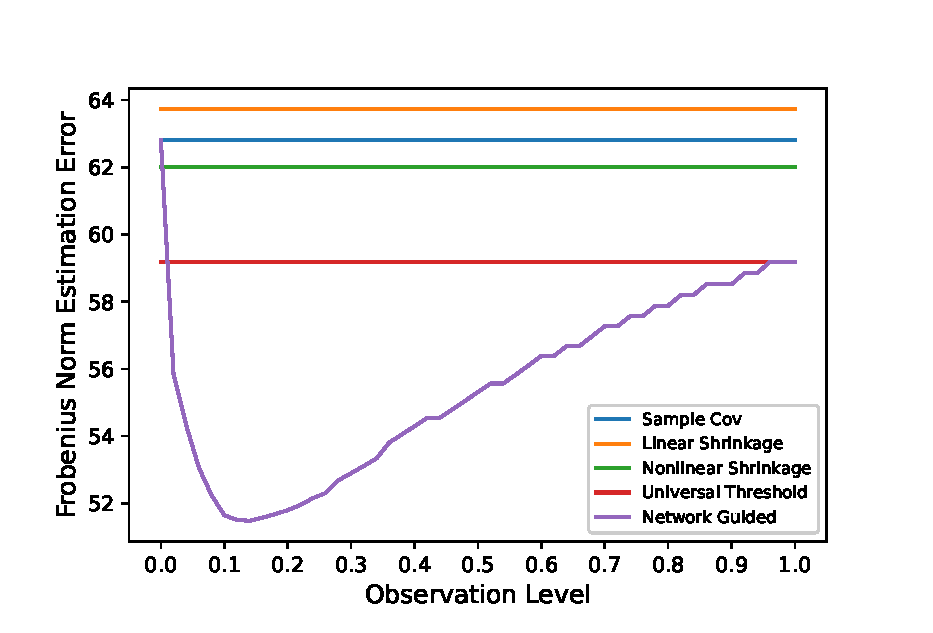
\includegraphics{Covariance-Estimation-with-Auxiliary-Information/asset/observation-level.eps}
     \caption{The estimation error against the observation level}
     \label{fig:1}
\end{figure}
when we set observation level equal to \(0\), the network guided estimator will be the same as the sample covariance estimator, on the other extreme, when observation level is set to \(1\), the network guided estimator is equivalent to universal thresholding. In between these cases, when we have information about the locations of the important pairs, we have a range where the estimation error is lowered. 

\begin{longtable}{lrrrrrrrrrrr}
\caption{The estimation error of the Network Guided Estimator with varying probabilities $p$, $q$ that determine how $G$ is generated.}
\label{t:3}\\
\toprule
q &   0.0 &   0.1 &   0.2 &   0.3 &   0.4 &   0.5 &   0.6 &   0.7 &   0.8 &   0.9 &   1.0 \\
p   &       &       &       &       &       &       &       &       &       &       &       \\
\midrule
\endfirsthead
\caption[]{The estimation error of the Network Guided Estimator with varying probabilities $p$, $q$ that determine how $G$ is generated.} \\
\toprule
q &   0.0 &   0.1 &   0.2 &   0.3 &   0.4 &   0.5 &   0.6 &   0.7 &   0.8 &   0.9 &   1.0 \\
p   &       &       &       &       &       &       &       &       &       &       &       \\
\midrule
\endhead
\midrule
\multicolumn{12}{r}{{Continued on next page}} \\
\midrule
\endfoot

\bottomrule
\endlastfoot
0.0 & 29.87 & 29.32 & 29.04 & 28.81 & 28.60 & 28.92 & 29.11 & 29.69 & 30.35 & 30.90 & 31.64 \\
0.1 & 28.80 & 28.27 & 27.90 & 27.78 & 27.78 & 27.88 & 28.26 & 28.76 & 29.37 & 29.99 & 30.74 \\
0.2 & 27.81 & 27.27 & 27.05 & 26.68 & 26.73 & 26.90 & 27.15 & 27.79 & 28.40 & 28.96 & 29.77 \\
0.3 & 26.79 & 26.26 & 25.99 & 25.66 & 25.80 & 25.84 & 26.23 & 26.71 & 27.45 & 28.20 & 28.94 \\
0.4 & 25.72 & 25.29 & 24.95 & 24.64 & 24.70 & 24.96 & 25.25 & 25.90 & 26.64 & 27.37 & 28.05 \\
0.5 & 24.68 & 24.20 & 24.04 & 23.84 & 23.86 & 23.94 & 24.54 & 24.91 & 25.59 & 26.34 & 27.02 \\
0.6 & 23.85 & 23.47 & 23.03 & 22.92 & 22.91 & 23.03 & 23.52 & 24.54 & 25.35 & 26.21 & 27.07 \\
0.7 & 22.87 & 22.58 & 22.17 & 22.00 & 22.18 & 23.06 & 23.82 & 24.85 & 25.63 & 26.51 & 27.44 \\
0.8 & 21.85 & 21.54 & 21.30 & 21.67 & 22.44 & 23.53 & 24.25 & 25.10 & 26.06 & 26.89 & 27.83 \\
0.9 & 20.99 & 20.76 & 21.36 & 22.17 & 22.79 & 23.77 & 24.64 & 25.59 & 26.46 & 27.33 & 28.21 \\
1.0 & 20.36 & 21.08 & 21.85 & 22.62 & 23.42 & 24.06 & 25.07 & 25.95 & 26.73 & 27.76 & 28.66 \\
\end{longtable}


In \autoref{t:3}, we have when \(p = q = 0\) the estimation error of the universal thresholding estimator, and \(p =q =1\) the sample covaraince estimation error. As we can see, as long as \(q\) is not large, the estimation error will be smaller when we have a higher probability \(p\) of observing the true large elements. It should be noted that \(q\) in fact cannot be very large, given that the whole matrix is sparse. 


